\documentclass[a4paper, 14pt]{extarticle}

\usepackage{../latexDependencies/misc/preamble2}

\geometry{a4paper}

% Название дисциплины
\newcommand{\subject}{Теория вероятности и математическая статистика} 

% Тип работы
% lab - для лабораторной работы 
% hw  - для домашней     работы
\newcommand{\task}{lab} 

% Номер работы
\newcommand{\taskNumber}{8} 

% Название работы
\newcommand{\taskNameOne}{Применение критерия $\chi^2$ Пирсона} 
\newcommand{\taskNameTwo}{к проверке гипотезы о виде функции распределения} 

% Имя студента
\newcommand{\studentName}{Очкин Н.В.}

% Имя преподававателя
\newcommand{\teacherName}{Облакова Т.В.}

% Группа
\newcommand{\group}{ФН11-52Б}

% Вариант
\newcommand{\variant}{9}

\begin{document}

\graphicspath{ {../latexDependencies/images} } 
\normalsize

\newcommand{\printTask}{%
    \ifthenelse{\equal{\task}{lab}}{%
        лабораторной%
    }{%
        \ifthenelse{\equal{\task}{hw}}{%
            домашней%
        }{%
            Неизвестный тип задания%
        }%
    }%
}

\begin{titlepage}

    \begin{center}
        {\footnotesize \itshape Федеральное государственное бюджетное 
                       образовательное учреждение высшего образования}
    \end{center}

    \begin{minipage}[c]{0.1\textwidth}
        
\includegraphics[width=1.1\textwidth]{iconBMSTU}
    \end{minipage}
    \hfill
    \begin{minipage}[c]{0.9\textwidth}
        \centering
        \itshape
        \bfseries
        \small
        \guillemotleft Московский государственный технический университет \\
        имени Н.Э. Баумана\guillemotright \\
        (национальный исследовательский университет) \\
        (МГТУ им. Н.Э. Баумана) 
    \end{minipage}

    \vspace{0.5cm}
    \noindent\rule{\textwidth}{2pt} \\

    \noindent\uline{\textbf{ФАКУЛЬТЕТ} ФУНДАМЕНТАЛЬНЫЕ НАУКИ} \\
    \vspace{-5pt} \\
    \noindent\uline{\textbf{КАФЕДРА} ВЫЧИСЛИТЕЛЬНАЯ МАТЕМАТИКА И МАТЕМАТИЧЕСКАЯ} \\
    \vspace{-5pt} \\
    \noindent\uline{ФИЗИКА (ФН11)} \\
    \vspace{-5pt} \\
    \noindent\uline{\textbf{НАПРАВЛЕНИЕ ПОДГОТОВКИ} МАТЕМАТИКА И КОМПЬЮТЕРНЫЕ} \\
    \vspace{-5pt} \\
    \noindent\uline{НАУКИ (02.03.01)} \\

    \begin{center}
        \bfseries
        \textsc{О т ч е т} \\[10pt]
        по \printTask {} работе \textnumero {} \taskNumber
    \end{center}

    \vspace{10pt}

    \hspace{10pt} 
    \noindent \textbf{Название \printTask {} работы:} \par
    \vspace{5pt}
    \hspace{10pt} 
    \noindent \textbf{\uline{\taskNameOne}} \vspace{5pt} \\
    \null\hspace{31pt} 
    \textbf{\uline{\taskNameTwo}} \vspace{5pt} 

    \vspace{10pt}

    \begin{center}
        \bfseries
        Вариант \textnumero {} \variant
    \end{center}

    \vspace{20pt}

    \hspace{10pt} 
    \noindent \textbf{Дисциплина:} \par
    \vspace{10pt}
    \hspace{10pt} 
    \noindent {\large \subject}

    \vspace{10pt}

    \begin{flushright}
        \renewcommand{\arraystretch}{3}
        \begin{tabular}{r r r}
            \multicolumn{1}{l}{Студент группы \uline{\group}} & 
            $\quad \underset{\text{(Подпись, дата)}}{\underline{\hspace{3cm}}} \quad$ & 
            \multicolumn{1}{c}{$\underset{\text{(И.О. Фамилия)}}{\uline{\textbf{\studentName}}}$} \\

            \multicolumn{1}{l}{Преподаватель} & 
            $\quad \underset{\text{(Подпись, дата)}}{\underline{\hspace{3cm}}} \quad$ & 
            \multicolumn{1}{c}{$\underset{\text{(И.О. Фамилия)}}{\uline{\textbf{\teacherName}}}$} \\
        \end{tabular}
    \end{flushright}

    \vfill

    \begin{center}
        \small
        Москва, 2024
    \end{center}
\end{titlepage}


\newgeometry{left=25mm, right=25mm, top=20mm, bottom=20mm}

\graphicspath{ {../latexDependencies/images/LW8} }

% Customize section, subsection, subsubsection and paragraph styles
\titleformat{\section}
  {\normalfont\large\bfseries}{\thesection}{1em}{}

\titleformat{\subsection}
  {\normalfont\normalsize\bfseries}{\thesubsection}{1em}{}

\titleformat{\subsubsection}
  {\normalfont\small\bfseries}{\thesubsubsection}{1em}{}

\titleformat{\paragraph}
  {\small\small\bfseries}{\theparagraph}{1em}{}

\thispagestyle{empty}

\null\newpage

% \setcounter{tocdepth}{5}
% \setcounter{secnumdepth}{5}

% \pagenumbering{roman}

% \tableofcontents
% \newpage

\pagenumbering{arabic}
\setcounter{page}{1}

\setstretch{1}
\linespread{1.1}

\setlength{\parindent}{0pt}

\fontsize{12pt}{16pt}\selectfont

\definecolor{myblue}{HTML}{0A88C2}
\definecolor{myred}{HTML}{FF1B1C}
\definecolor{mygreen}{HTML}{386641}

\lstdefinestyle{mystyle}{
    basicstyle=\ttfamily\footnotesize,
    keywordstyle=\color{myblue},
    stringstyle=\color{myred},
    commentstyle=\color{green!50!black},
    showstringspaces=false,
    frame=leftline, 
    framesep=10pt, 
}

% Set the style for Python code
\lstset{style=mystyle, extendedchars=\true}

% --------------------------------------START--------------------------------------

\section*{Задание}\vspace{-20pt}\rule{\linewidth}{0.1mm}

\begin{enumerate}
    \item Используя группированную выборку из задачи $\textnumero 1$, проверьте на уровне $\alpha$ гипотезу $H_0$: выборка взята из генеральной совокупности, распределенной по закону $F(x)$.
    \item Неизвестные параметры распределения $F(x)$, если это необходимо, найдите методом моментов или методом максимального правдоподобия по выборке.
    \item Постройте совмещенные графики гистограммы относительных частот и плотности, соответствующей функции распределения $F(x)$.
    \item Дайте анализ полученного решения.
\end{enumerate}

\section*{Исходные данные}\vspace{-20pt}\rule{\linewidth}{0.1mm}

\begin{equation*}
    \text{R}[\text{a, b}] \qquad \alpha = 0.01
\end{equation*}

\vspace{-20pt}

\begin{equation*}
    \begin{vmatrix}
        14.495 & 4.715 & 7.175 & 8.428 & 11.093 & 3.375 & 12.906 & 8.415 & 8.916 & 13.48 \\
        5.343 & 17.985 & 15.992 & 13.89 & 9.838 & 13.924 & 9.012 & 9.458 & 17.69 & 6.542 \\
        14.396 & 8.592 & 8.206 & 14.237 & 7.357 & 10.821 & 12.767 & 16.058 & 12.959 & 4.354 \\
        12.888 & 10.268 & 9.182 & 5.647 & 8.282 & 2.903 & 15.988 & 12.959 & 14.919 & 6.339 \\
        2.375 & 17.921 & 9.097 & 15.85 & 11.449 & 11.095 & 9.493 & 12.175 & 7.479 & 13.535 \\
        9.234 & 6.078 & 4.964 & 6.355 & 13.957 & 12.911 & 15.694 & 14.286 & 9.869 & 5.175 \\
        5.811 & 7.241 & 5.814 & 3.086 & 6.875 & 3.878 & 5.333 & 15.134 & 12.924 & 9.159 \\
        4.727 & 4.646 & 15.535 & 9.919 & 17.117 & 10.351 & 16.892 & 12.423 & 10.511 & 4.942 \\
        4.843 & 9.927 & 15.864 & 3.635 & 17.963 & 8.25 & 5.14 & 6.734 & 12.622 & 13.325 \\
        3.377 & 16.195 & 12.04 & 12.768 & 2.744 & 14.186 & 9.354 & 15.439 & 14.612 & 15.649 \\
    \end{vmatrix}
\end{equation*}

Сгруппируем данные:

\begin{center}
  \begin{lstlisting}[language=Python]
def group(data):
    n_ = len(data)

    min_ = min(data)
    max_ = max(data)

    range_ = max_ - min_

    l_ = 1 + int(np.log2(n_))

    h_ = range_ / l_

    int_boundaries_ = np.array(
        [min_ + i * h_ for i in range(0, l_ + 1, 1)]
    )
    intervals_ = np.array(
        [(int_boundaries_[i], int_boundaries_[i+1]) for i in range(0, l_, 1)]
    )
    mid_ranges_ = np.array(
        [sum(interval)/2 for interval in intervals_]
    )

    present = lambda el, int_ : int_[0] <= el < int_[1]
    freqs_ = np.zeros(l_)
    for el in data:
        for j in range(0, l_, 1):
            if present(el, intervals_[j]):
                freqs_[j] += 1 

    freqs_[-1] += np.count_nonzero(data == max_)

    rel_freqs_ = freqs_ / n_

    rel_freqs_density_ = rel_freqs_ / h_

    return n_, \
           min_, \
           max_, \
           range_, \
           l_, \
           h_, \
           int_boundaries_, \
           intervals_, \
           mid_ranges_, \
           freqs_, \
           rel_freqs_, \
           rel_freqs_density_

n_, \
min_, \
max_, \
range_, \
l_, \
h_, \
int_boundaries_, \
intervals_, \
mid_ranges_, \
freqs_, \
rel_freqs_, \
rel_freqs_density_ = group(data_)
  \end{lstlisting}
\end{center}

\begin{center}
    \renewcommand{\arraystretch}{1.5}
    \begin{tabular}{ll}
        \toprule
        \textbf{Параметр} & \textbf{Значение} \\
        \midrule
        Количество наблюдений, \( n \) & 120 \\
        Минимальное значение & 2.375 \\
        Максимальное значение & 17.985 \\
        Размах & 15.61 \\
        Количество интервалов, \( l \) & 7 \\
        Ширина интервала, \( h \) & 2.23 \\
        \bottomrule
    \end{tabular}
\end{center}

\begin{center}
    \begin{adjustbox}{max width=1\textwidth}
    \renewcommand{\arraystretch}{1.5}
    \begin{tabular}{cccccc}
        \toprule
        \textbf{Границы}    & \textbf{Интервалы} & \textbf{Середины} & \textbf{Частоты} & \textbf{Относительные} & \textbf{Плотность} \\
        \textbf{интервалов} &                    &                   &                  &                        & \textbf{относительных} \\
                            &                    &                   &                  & \textbf{частоты}       & \textbf{частот} \\
        \midrule
        2.375 & [2.375, 4.605] & 3.49 & 12 & 0.1 & 0.04484305 \\
        4.605 & [4.605, 6.835] & 5.72 & 20 & 0.167 & 0.07473842 \\
        6.835 & [6.835, 9.065] & 7.95 & 18 & 0.15 & 0.06726457 \\
        9.065 & [9.065, 11.295] & 10.18 & 18 & 0.15 & 0.06726457 \\
        11.295 & [11.295, 13.525] & 12.41 & 17 & 0.14167 & 0.06352765 \\
        13.525 & [13.525, 15.755] & 14.64 & 20 & 0.167 & 0.07473842 \\
        15.755 & [15.755, 17.985] & 16.87 & 14 & 0.1167 & 0.05231689 \\
        17.985 &                  &       &    &        &            \\
        \bottomrule
    \end{tabular}
    \end{adjustbox}
\end{center}

Оценим параметры:

\vspace{-20pt}

\begin{gather*}
    \text{a} = \text{min} = 2.375 \\
    \text{b} = \text{max} = 17.985 
\end{gather*}

Найдем $\chi^2_{\text{в}}$:

\begin{equation*}
    \chi^2_{\text{в}} = \sum_{i=1}^{l} \cfrac{(\nu_i - n p_i)^2}{n p_i}
\end{equation*}

Количество значений, попавших в j-ый интервал группировки ($\nu$) нам уже известно и 
записано в столбце \textbf{Частоты} в таблице выше. \\

\newpage

Определим теоретическую вероятность попадания в j-ый интервал группировки ($p$):

\begin{center}
    \begin{lstlisting}[language=Python]
theorIntHitProbs_  = [] # p_j
theorIntHitProbsN_ = [] # n*p_j

cdf_ = lambda x : sp.stats.uniform.cdf(x, loc=a, scale=b-a)

for interval in intervals_:
    beg = interval[0]
    end = interval[1]

    theorIntHitProb = cdf_(end) - cdf_(beg)
    theorIntHitProbs_.append(theorIntHitProb)

    theorIntHitProbsN_.append(n_ * theorIntHitProb)
    \end{lstlisting}
\end{center}

\vspace{-20pt}

\begin{flalign*}
    & p_i: [0.143 \hspace{10pt} 0.143 \hspace{10pt} 0.143 \hspace{10pt} 0.143 \hspace{10pt} 0.143 \hspace{10pt} 0.143 \hspace{10pt} 0.143] \\
    & n \cdot p_i: [17.143 \hspace{10pt} 17.143 \hspace{10pt} 17.143 \hspace{10pt} 17.143 \hspace{10pt} 17.143 \hspace{10pt} 17.143 \hspace{10pt} 17.143] \\
\end{flalign*}

\vspace{-30pt}

\begin{equation*}
    \text{sum}(p) == 1
\end{equation*}
  
Итого имеем:

\begin{center}
    \begin{lstlisting}[language=Python]
Chi2_v = sum([((freqs_[i] - theorIntHitProbsN_[i])**2) / \
                    theorIntHitProbsN_[i] for i in range(l_)])
    \end{lstlisting}
\end{center}

\vspace{-20pt}

\begin{equation*}
    \chi^2_{\text{в}} \approx 3.1583
\end{equation*}

\vspace{10pt}

Теперь определим квантиль с $l - 1 - 2 = 4$ степенями свободы:

\begin{center}
    \begin{lstlisting}[language=Python]
quantile = sp.stats.chi2.ppf(1 - alpha_, l_ - 1 - 2)
    \end{lstlisting}
\end{center}

\vspace{-20pt}

\begin{equation*}
    \chi_{1 - \alpha}^2 (l - 1 - 2) = \chi_{0.99}^2 (4) \approx 13.2767
\end{equation*}

\begin{equation*}
    \chi^2_{\text{в}} < \chi_{0.99}^2 (4) \Rightarrow \text{гипотеза принимается}
\end{equation*}

\vspace{10pt}

Построим совмещенные графики гистограммы относительных частот и плотности, 
соответствующей функции непрерывного равномерного распределения с 
параметрами a = 2.375 и b = 17.985.

\begin{center}
    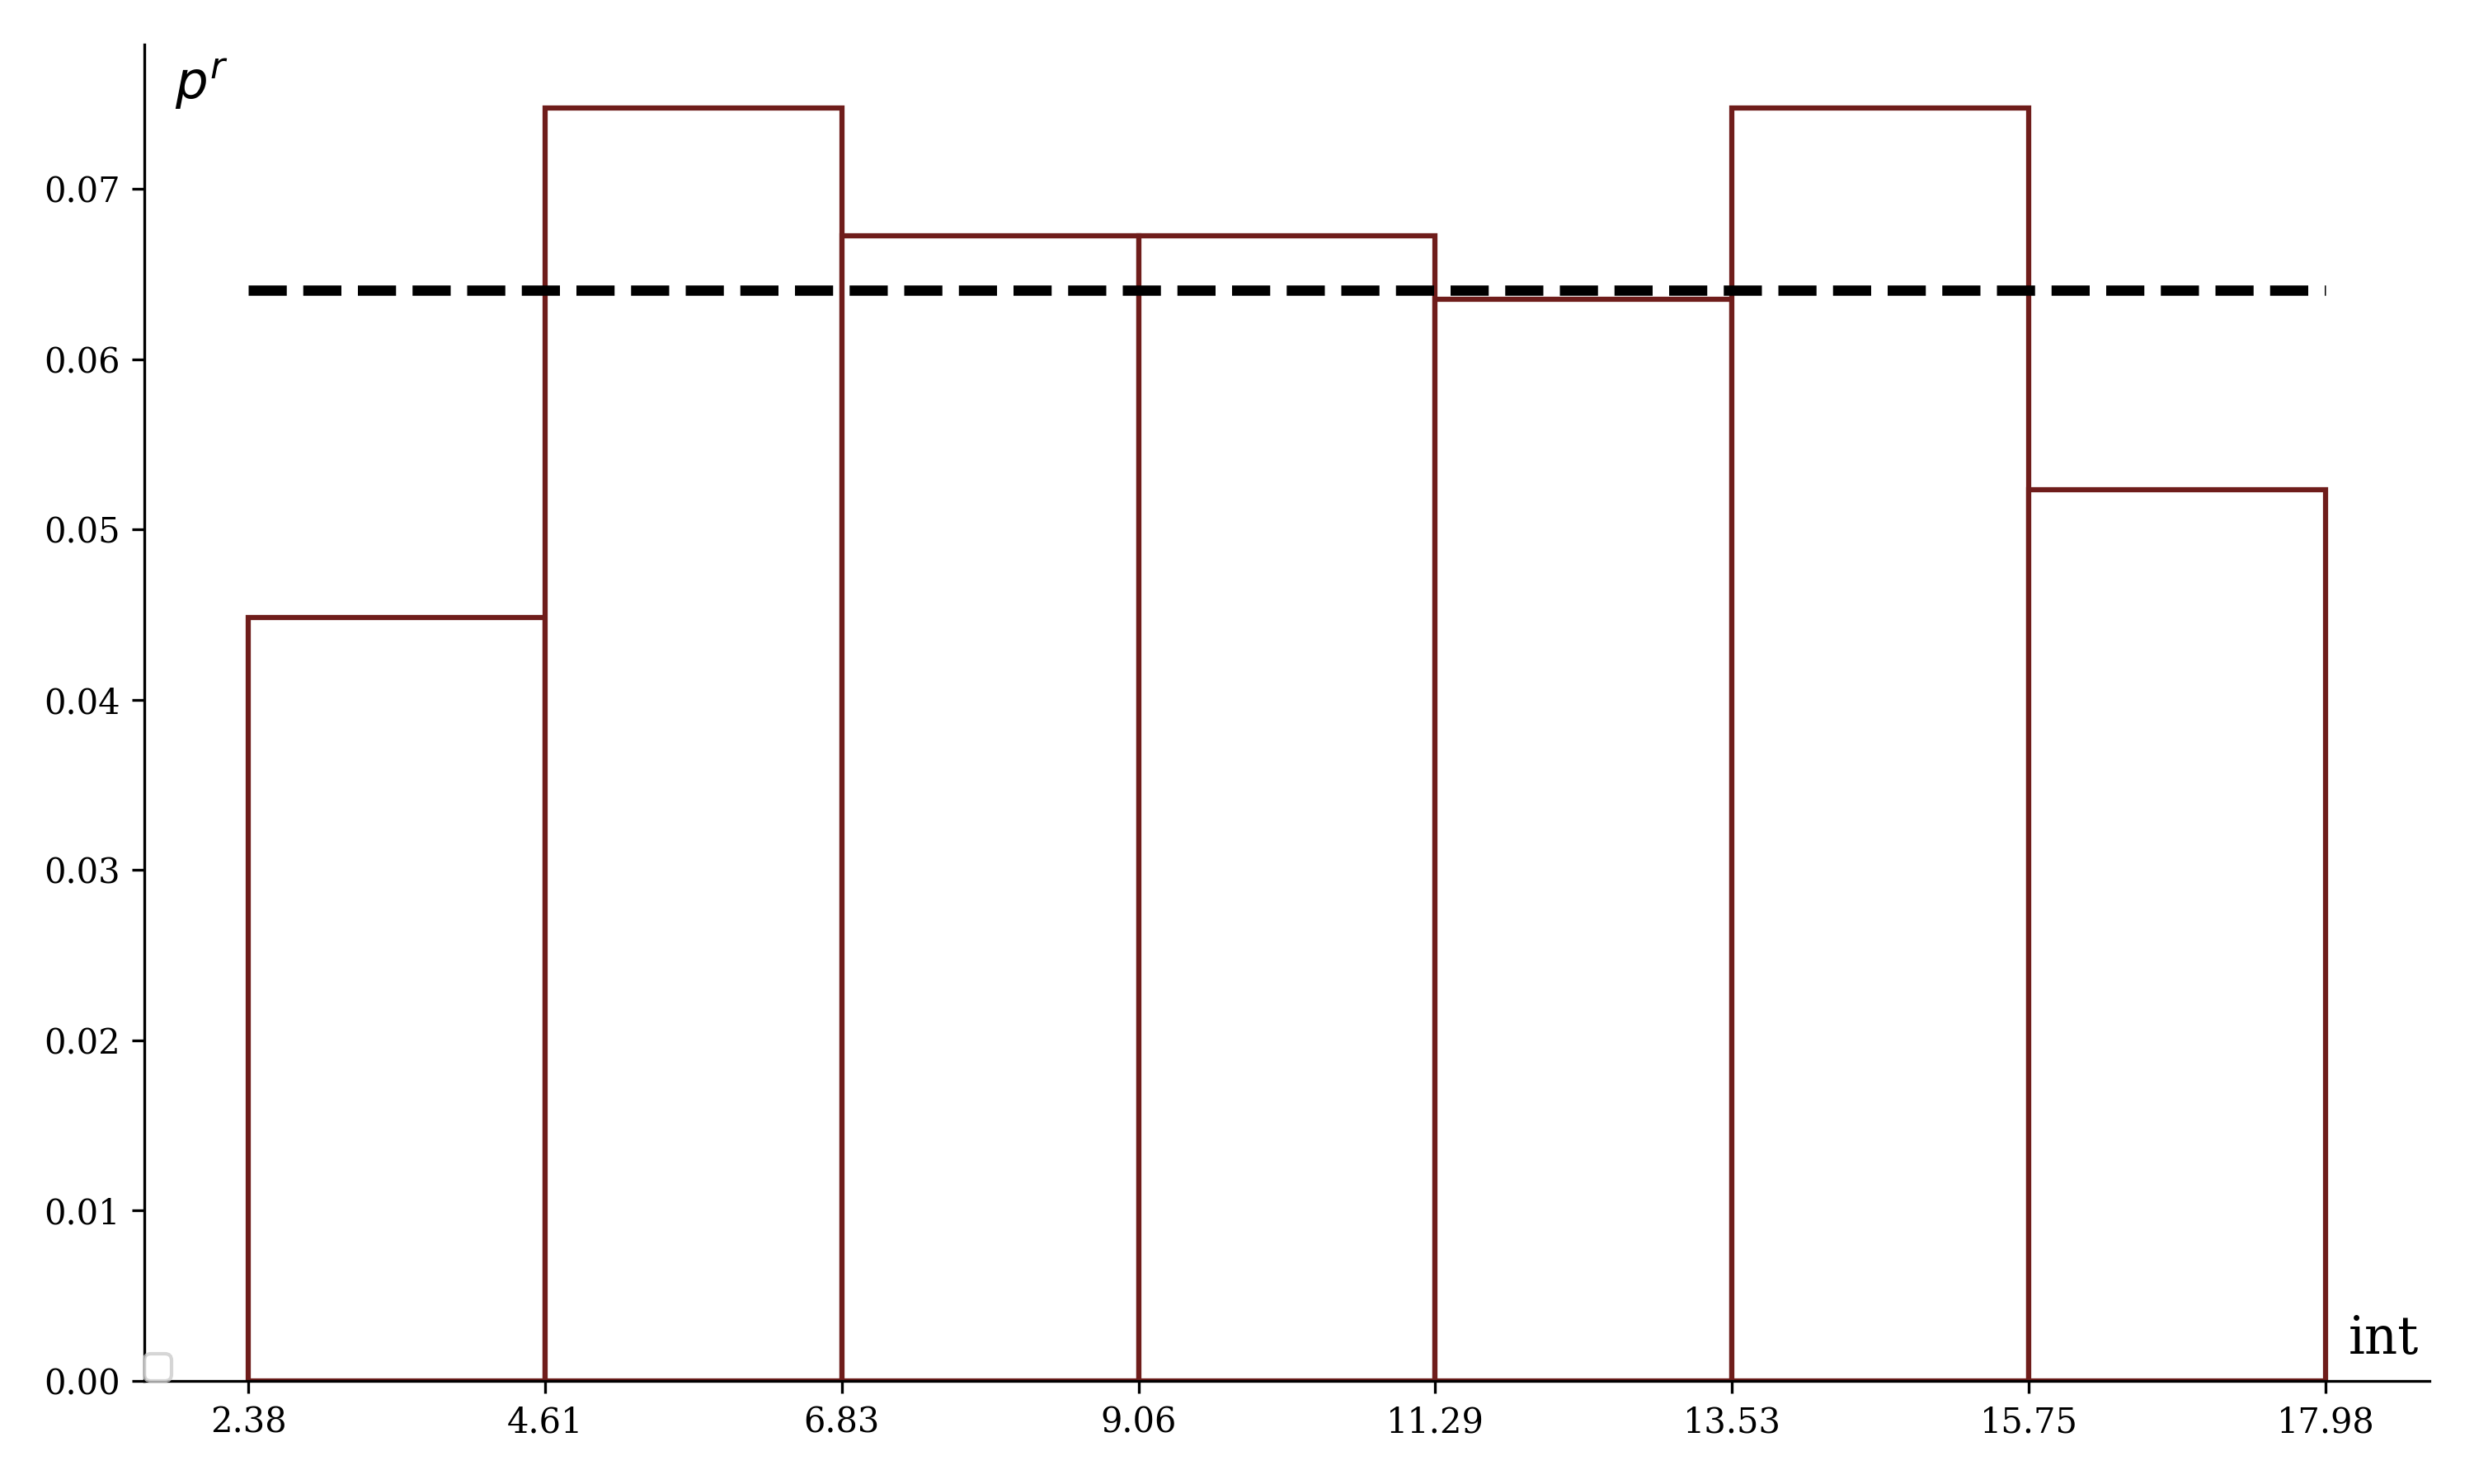
\includegraphics[width=\textwidth, height=\textheight, keepaspectratio]{hist} \\
\end{center}

\section*{Вывод}\vspace{-20pt}\rule{\linewidth}{0.1mm}

В ходе выполнения лабораторной работы были перепроверены выводы, 
сделанные в первой лабораторной работе, и действительно показано, 
что на уровне доверия $\alpha = 0.01$ выборка взята из генеральной совокупности, 
распределенной по непрерывному нормальному закону с найденными 
параметрами a и b.

% ---------------------------------------CODE---------------------------------------

\newpage

\section*{Приложение}\vspace{-20pt}\rule{\linewidth}{0.1mm}

Программный код, с помощью которого была выполнена данная лабораторная работа.\\

\begin{center}
    \begin{lstlisting}[language=Python]
import numpy as np
import scipy as sp
import matplotlib.pyplot as plt

alpha_ = 0.01

data_ = [
    14.495, 4.715, 7.175, 8.428, 11.093, 3.375, 12.906, 8.415, 8.916, 13.48,
    5.343, 17.985, 15.992, 13.89, 9.838, 13.924, 9.012, 9.458, 17.69, 6.542,
    14.396, 8.592, 8.206, 14.237, 7.357, 10.821, 12.767, 16.058, 12.959, 4.354,
    12.888, 10.268, 9.182, 5.647, 8.282, 2.903, 15.988, 12.959, 14.919, 6.339,
    2.375, 17.921, 9.097, 15.85, 11.449, 11.095, 9.493, 12.175, 7.479, 13.535,
    9.234, 6.078, 4.964, 6.355, 13.957, 12.911, 15.694, 14.286, 9.869, 5.175,
    5.811, 7.241, 5.814, 3.086, 6.875, 3.878, 5.333, 15.134, 12.924, 9.159,
    4.727, 4.646, 15.535, 9.919, 17.117, 10.351, 16.892, 12.423, 10.511, 4.942,
    4.843, 9.927, 15.864, 3.635, 17.963, 8.25, 5.14, 6.734, 12.622, 13.325,
    3.377, 16.195, 12.04, 12.768, 2.744, 14.186, 9.354, 15.439, 14.612, 15.649,
    8.681, 5.006, 3.608, 2.867, 12.177, 15.506, 7.683, 14.022, 17.103, 8.905,
    12.173, 17.757, 6.883, 2.666, 9.861, 5.743, 16.175, 15.308, 7.039, 15.238
]

def decorate_plot(ax, x_ticks, xname, yname, loc=(-0.025, -0.3)):
    SIZE_TICKS = 10

    # Eliminate upper and right axes
    ax.spines['right'].set_color('none')
    ax.spines['top'].set_color('none')

    # Show ticks in the left and lower axes only
    ax.xaxis.set_ticks_position('bottom')
    ax.yaxis.set_ticks_position('left')

    # axis names
    ax.set_xlabel(xname, fontsize=15)
    ax.xaxis.set_label_coords(0.98, 0.05)

    ax.set_ylabel(yname, rotation=0, fontsize=15)
    ax.yaxis.set_label_coords(0.025, 0.95)

    ax.set_xticks(x_ticks)

    # Adjust the font size of the tick labels
    ax.tick_params(axis='both', which='major', labelsize=SIZE_TICKS)

    plt.legend(fontsize=10, loc=loc)

    # Update font settings
    plt.rcParams.update({'font.family': 'serif', 'font.size': 12})

    # Adjust layout
    plt.tight_layout()

def clean(data):
    res = []
    for el in data:
        res.append(round(el, 3))
    return res

def group(data):
    n_ = len(data)
    print(f'n: {n_}')

    min_ = min(data)
    max_ = max(data)
    print(f'min: {min_}     max: {max_}')

    range_ = max_ - min_
    print(f'range: {range_}')

    l_ = 1 + int(np.log2(n_))
    print(f'l: {l_}')

    h_ = range_ / l_
    print(f'h: {h_}')

    int_boundaries_ = np.array(
        [min_ + i * h_ for i in range(0, l_ + 1, 1)]
    )
    print(f'interval boundaries: {int_boundaries_}')
    intervals_ = np.array(
        [(int_boundaries_[i], int_boundaries_[i+1]) for i in range(0, l_, 1)]
    )
    print(f'intervals: {intervals_}')
    mid_ranges_ = np.array(
        [sum(interval)/2 for interval in intervals_]
    )
    print(f'intervals\' midpoints: {mid_ranges_}')

    present = lambda el, int_ : int_[0] <= el < int_[1]
    freqs_ = np.zeros(l_)
    for el in data:
        for j in range(0, l_, 1):
            if present(el, intervals_[j]):
                freqs_[j] += 1 

    freqs_[-1] += np.count_nonzero(data == max_)
    print(f'frequencies: {freqs_}')

    rel_freqs_ = freqs_ / n_
    print(f'relative frequencies: {rel_freqs_}')

    rel_freqs_density_ = rel_freqs_ / h_
    print(f'relative frequencies\' density: {rel_freqs_density_}')

    print(f'-'*100)

    space_ = ' ' * 5
    for i in range(l_):
        print(f'{intervals_[i]}{space_}{freqs_[i]}{space_}{rel_freqs_[i]}{space_}{rel_freqs_density_[i]}')
    
    return n_, \
           min_, \
           max_, \
           range_, \
           l_, \
           h_, \
           int_boundaries_, \
           intervals_, \
           mid_ranges_, \
           freqs_, \
           rel_freqs_, \
           rel_freqs_density_

n_, \
min_, \
max_, \
range_, \
l_, \
h_, \
int_boundaries_, \
intervals_, \
mid_ranges_, \
freqs_, \
rel_freqs_, \
rel_freqs_density_ = group(data_)

a = min_
b = max_

theorIntHitProbs_  = [] # p_j
theorIntHitProbsN_ = [] # n*p_j

cdf_ = lambda x : sp.stats.uniform.cdf(x, loc=a, scale=b-a)

for interval in intervals_:
    beg = interval[0]
    end = interval[1]

    theorIntHitProb = cdf_(end) - cdf_(beg)
    theorIntHitProbs_.append(theorIntHitProb)

    theorIntHitProbsN_.append(n_ * theorIntHitProb)

print(f'p_i: {clean(theorIntHitProbs_)}')
print(f'n * p_i: {clean(theorIntHitProbsN_)}')

sum(theorIntHitProbs_)

Chi2_v = sum([((freqs_[i] - theorIntHitProbsN_[i])**2)/theorIntHitProbsN_[i] for i in range(l_)])
Chi2_v

quantile = sp.stats.chi2.ppf(1 - alpha_, l_ - 1 - 2)
quantile

def buildBar(filename):
    RED = '#6F1D1B'

    _, ax = plt.subplots(figsize=(10, 6))

    x_values = mid_ranges_
    y_values = rel_freqs_density_

    ax.bar(x_values, 
           y_values, 
           width=h_, 
           color='white',
           edgecolor=RED, 
           linestyle='-', 
           linewidth=1.5, 
           align='center')
    
    x_values = np.linspace(min_, max_, 100)
    y_values = sp.stats.uniform.pdf(x_values, loc=a, scale=b-a)
    ax.plot(x_values, 
            y_values, 
            color='black',
            linestyle='--', 
            linewidth=3)

    decorate_plot(ax, int_boundaries_, 'int', '$p^r$', loc=(0, 0))

    plt.savefig(f'{filename}.png', dpi=300, transparent=True)

    plt.show()

buildBar('hist')
    \end{lstlisting}
\end{center}

\end{document}
